%%%%%%%%%%%%%%%%%%%%%%%%%%%%%%%%%%%%%%%%%
% Friggeri Resume/CV
% XeLaTeX Template
% Version 1.2 (3/5/15)
%
% This template has been downloaded from:
% http://www.LaTeXTemplates.com
%
% Original author:
% Adrien Friggeri (adrien@friggeri.net)
% https://github.com/afriggeri/CV
%
% License:
% CC BY-NC-SA 3.0 (http://creativecommons.org/licenses/by-nc-sa/3.0/)
%
% Important notes:
% This template needs to be compiled with XeLaTeX and the bibliography, if used,
% needs to be compiled with biber rather than bibtex.
%
%%%%%%%%%%%%%%%%%%%%%%%%%%%%%%%%%%%%%%%%%

\documentclass[]{friggeri-cv} % Add 'print' as an option into the square bracket to remove colors from this template for printing

\addbibresource{llevitiscv.bib} % Specify the bibliography file to include publications

\begin{document}

\header{elizabeth}{levitis}{PhD Candidate} % Your name and current job title/field

%----------------------------------------------------------------------------------------
%	SIDEBAR SECTION
%----------------------------------------------------------------------------------------

\begin{aside} % In the aside, each new line forces a line break
 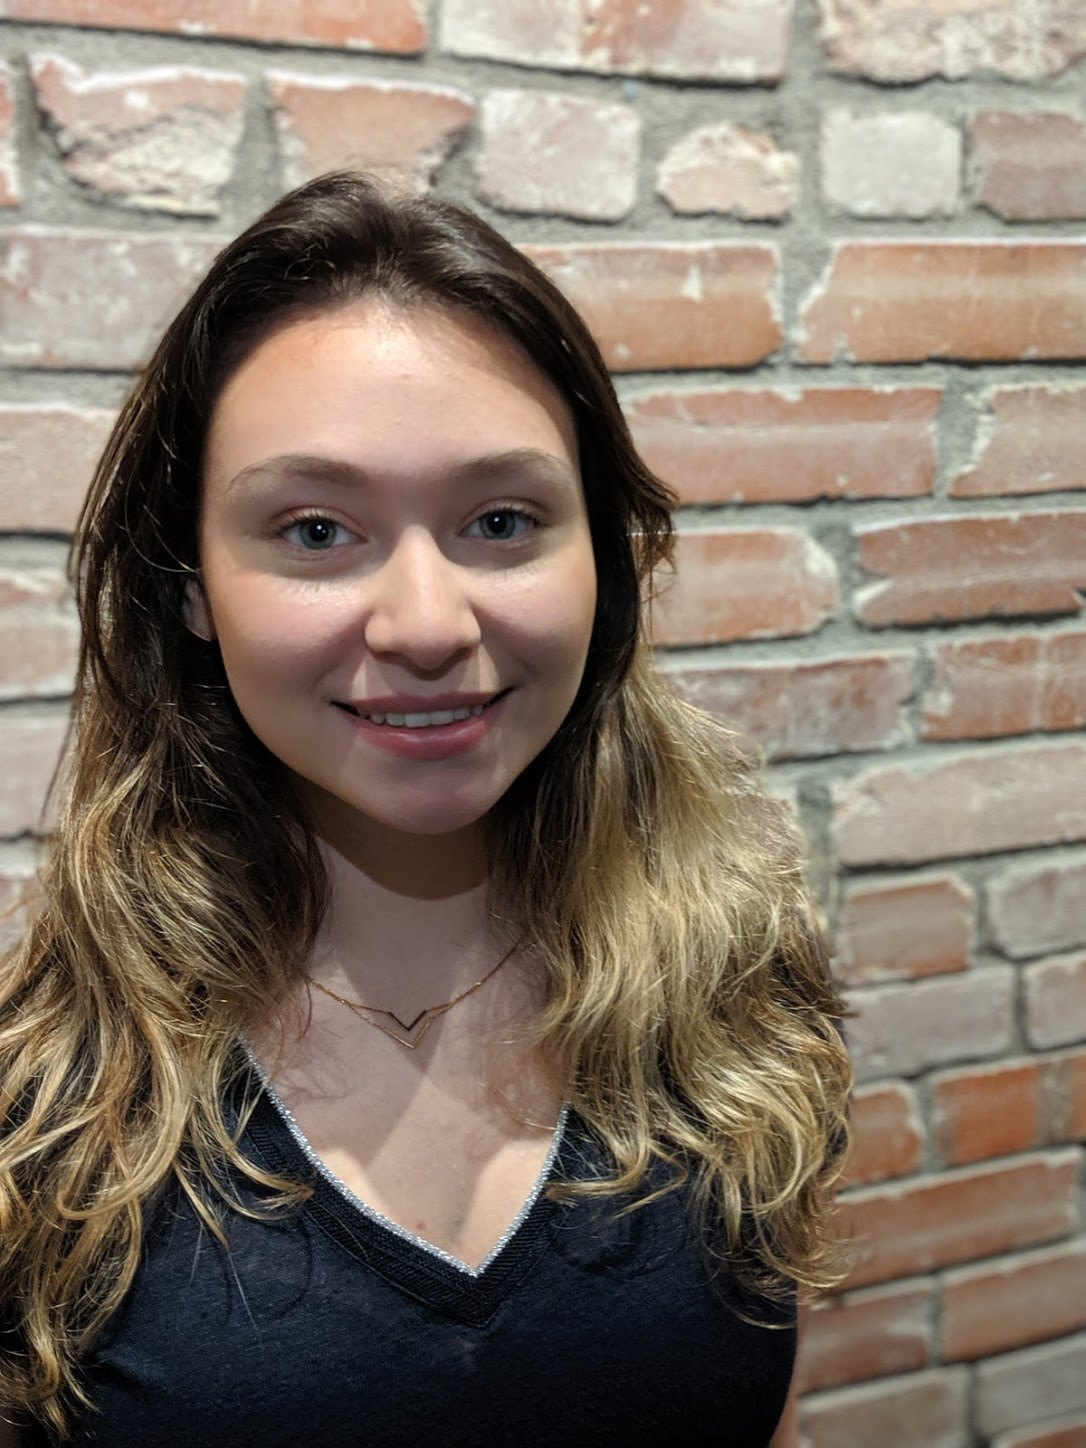
\includegraphics[width=\textwidth]{./llevitis_headshot.jpg}
\section{contact}
\href{mailto:elizabeth.levitis@mail.mcgill.ca}{elizabeth.levitis\\@nih.gov~{\color{red} \faEnvelope}}
\href{http://github.com/llevitis}{llevitis~{\color{purple} \faGithub}}
\href{https://twitter.com/LevitisLiza}{LevitisLiza~{\color{blue} \faTwitter}}%\href{http://orcid.org/0000-0001-8915-496X}{{\color{orcidgreen} \aiOrcid}} %\href{https://scholar.google.com/citations?user=ztw6g7kAAAAJ&hl=en}{{\color{googred} \aiGoogleScholar}} %\href{https://www.researchgate.net/profile/Gregory_Kiar}{{\color{gateteal} \aiResearchGate}}
\section{languages}
english native speaker,
russian native speaker,
basic spanish
\section{programming}
Python, R, Bash, PHP,
MATLAB, Javascript,
SQL, LaTeX, etc.
\section{soft skills}
problem~solving, teaching, leadership
\end{aside}

%----------------------------------------------------------------------------------------
%	EDUCATION SECTION
%----------------------------------------------------------------------------------------

\section{education}

\begin{entrylist}

%------------------------------------------------
\entry
{2020 -- now}
{Ph.D. candidate {\normalfont in Neuroscience}}
{University College London, London, United Kingdom | NIMH, Bethesda, MD, USA}
{UCL-NIMH Joint Doctoral Training Program in Neuroscience - supervised by Armin Raznahan (NIMH) and 
Daniel Alexander (UCL)}

\entry
{2018 -- 2020}
{M.Sc. {\normalfont in Neuroscience}}
{McGill University, Montreal, QC}
{Thesis work supervised by Alan C. Evans and Yasser Iturria-Medina on a project entitled:\\ 
Application of an Epidemic Spreading Model to Characterize Amyloid Beta Accumulation in Autosomal Dominant Alzheimer’s Disease Mutation Carriers.
}

\entry
{2013 -- 2017}
{B.A\&Sc {\normalfont in Cognitive Science}}
{McGill University, Montreal, QC}
{Thesis work was supervised by Veronique Bohbot on a project entitled:\\ 
Personality Measures Associated with Spatial and Response Learning Strategies
in Virtual Navigation}

%------------------------------------------------

\entry
{2019}
{ReproNim Instructor Training}
{ReproNim}
{Running workshops on reproducible neuroimaging.}

\end{entrylist}

%----------------------------------------------------------------------------------------
%	WORK EXPERIENCE SECTION
%----------------------------------------------------------------------------------------

\section{experience}

\subsection{Research Experience}

\begin{entrylist}

\entry
{07/20 -- now}
{Section on Developmental Neurogenomics, National Institute of Mental Health}
{Bethesda, MD}
{\job{Software Developer \& Researcher} \\
Applied best practices for reproducible neuroimaging to make existing datasets be Brain Imaging 
Data Structure compliant and processed multiple modalities with open-source image processing 
pipelines. Thesis work focuses on characterizing and predicting multimodal imaging phenotypes in individuals 
with sex chromosome aneuploidies.}

\entry
{05/17 -- 05/20}
{McGill Centre for Integrative Neuroscience (MCIN)}
{Montreal, QC}
{\job{Software Developer \& Researcher} \\
Involved in the ongoing development of a Quality Control module for imaging and
behavioral data, along with a standalone RESTful API for automatic structural MRI
quality control. Duties include developing new features for the Infant Brain Imaging
Study project. For thesis work I have contributed to the development of APPIAN, 
an automatic PET processing pipeline. My central thesis project focused on determining 
how sporadic and autosomal dominant Alzheimer's disease differ with regard to observed spreading 
patterns of amyloid beta.}    

\entry
{05 -- 08/16}
{Breast Cancer Informatics Group, McGill University}
{Montreal, QC}
{\job{Research Assistant}\\
Continued development of a supervised machine learning algorithm in R to predict
breast cancer patients' intrinsic subtypes across distinct subtyping schemes
using microarray data.}


\end{entrylist}
% % The "midamble" should be at the end of page 1
\input{midamble.tex}

\begin{entrylist}


\entry
{01/15 -- 06/15}
{Department of Biology, McGill University}
{Montreal, QC}
{\job{Work-Study Research Assistant}\\
Assisted with behavioral analysis of Zebra finch directed and undirected song
between an adult and juvenile. Gained histology experience using a sliding microtome
to section brain tissue and mount slices onto slides.}

\entry
{09/14 -- 12/14}
{Department of Psychology, McGill University}
{Montreal, QC}
{\job{Work-Study Research Assistant}\\
Carried out neuron quantification via cFos activation
in chick brains' slices using the software Stereo Investigator.
Performed microscopy work to determine neural density in 
coronal slices.
}


\entry
{10/13 -- 04/15}
{Department of Languages, Literature, and Culture, McGill University}
{Montreal, QC}
{\job{Work-Study Research Assistant}\\
Worked with a professor of Russian literature - tasks included translating Russian text and 
assisting with cross-referencing. 
}
\end{entrylist}

\subsection{Teaching Experience}

\begin{entrylist}

\entry
{09/20 -- 03/21}
{Florida International University}
{Miami, FL}
{\job{ABCD-ReproNim Teaching Assistant} \\
Contributed directly throughout the virtual online training course by providing support to students
during video presentations and answering questions in real-time via the website’s chat
feature and e-mail. Developed data exercises for weekly assignments, hosted weekly Q\&A sessions for enrolled students, 
and provided mentorship to students during the final project week.}


\entry
{01/18 -- 07/20}
{McGill University, OHBM, ReproNim, Brainhack}
{Montreal, QC}
{\job{Neuroinformatics Instructor} \\
Planning and teaching of workshops introducing neuroscientists and trainees to
topics pertaining to reproducible neuroimaging and neuroinformatics.}

\entry
{05/16 -- 07/16}
{McGill University}
{Montreal, QC}
{\job{Organic Chemistry Teaching Assistant} \\
Taught tutorials and helped grade exams for an intro to organic chemistry course.
}

\entry
{09/15 -- 12/16}
{McGill University}
{Montreal, QC}
{\job{Science Undergraduate Society Peer Tutor} \\
Tutored peers one-on-one in courses such as intro to computer science, intro to organic chemistry,
and developmental economics.
}

\entry
{07/15 -- 08/15}
{Hudson Guild}
{New York, NY}
{\job{SHSAT Instructor} \\
Planned and taught a month-long course to prepare a group of students to ace the SHSAT, 
an exam taken to gain admittance to the top high schools in NYC. Assessed students'
individual progress based on daily homework assignments and in-class participation.}

\end{entrylist}

% The "midamble" should be at the end of page 1
%\input{midamble.tex}

%----------------------------------------------------------------------------------------
%	EXTRACURRICULARS SECTION
%----------------------------------------------------------------------------------------
\section{memberships \& extracurriculars}

\begin{entrylist}
\entry
{2019 -- 2020}
{OHBM Open Science SIG}
{Minneapolis, MN}
{Hackathon Chair \& Organizer}

\entry
{2018 -- 2019}
{BrainReach}
{Montreal, QC}
{Neuroscience instructor for high school students \& course content developer}

\entry
{2016 -- 2017}
{McGill University Bachelor of Arts \& Science Integrative Council}
{Montreal, QC}
{Vice President (Academic)}

\end{entrylist}

\input{midamble.tex}

\begin{entrylist}

\entry
{2015 -- 2017}
{Swimability}
{Montreal, QC}
{Special Needs Swimming Instructor}

\entry
{2015 -- 2016}
{McGill Cognitive Science Student Association}
{Montreal, QC}
{Vice President (External)}
 
\entry
{2015 -- 2016}
{McGill Science Undergraduate Society}
{Montreal, QC}
{Peer Tutor}

\entry
{2014 -- 2015}
{Spoon University}
{Montreal, QC}
{Co-Founder \& Editor-in-Chief}
\end{entrylist}

%\newpage
%----------------------------------------------------------------------------------------
%	AWARDS SECTION
%----------------------------------------------------------------------------------------

\section{awards}

\begin{entrylist}
\vspace{-7pt}

\entry
{2020-2024}
{Pre-doctoral Intramural Research Training Award}
{National Institute of Mental Health, Bethesda, MD, USA}
{}
\vspace{-7pt}

\entry
{2019}
{Travel Award}
{Quebec Bio-imaging Network, Montreal, QC}
{}
\vspace{-7pt}

\entry
{2019}
{Instructor Training Fellowship}
{Repronim, Worcester, MA}
{}
\vspace{-7pt}
% $1000

\entry
{2017}
{Dean's Undergraduate Multidisciplinary Research Award}
{McGill University, Montreal, QC}
{}
\vspace{-7pt}

\entry
{2016}
{Undergraduate Research Award}
{McGill University, Montreal, QC}
{}
\vspace{-7pt}
% $10000

\entry
{2016}
{Tomlinson Engagement Award for Mentoring}
{McGill University, Montreal, QC}
{}
\vspace{-7pt}
% $300

\end{entrylist}

%----------------------------------------------------------------------------------------
%	INTERESTS SECTION
%----------------------------------------------------------------------------------------

\vspace{-7pt}
\section{interests}

\textbf{professional:} neuroscience, translational research, cognitive science,
informatics, software design, machine learning, statistics.
\textbf{personal:} dance, crossfit, cooking.

% \section{reviewed for}
% \begin{enumerate}
% \item Frontiers in Neuroinformatics
% \item Gigascience
% \end{enumerate}

%----------------------------------------------------------------------------------------
%	PUBLICATIONS SECTION
%----------------------------------------------------------------------------------------
% \clearpage

\section{publications}
\printbibsection{manual}{pre-prints} % Print all articles from the bibliography

\printbibsection{article}{articles in peer-reviewed journals} % Print all articles from the bibliography

\printbibsection{inproceedings}{proceedings in international peer-reviewed conferences} % Print all inproceedings entries from the bibliography

\printbibsection{inbook}{book chapters} % Print all inbook entires

\printbibsection{booklet}{invited talks \& organized workshops} % Print all booklet entries from the bibliography

\printbibsection{proceedings}{conference posters} % Print all proceedings entries from the bibliography

\printbibsection{report}{works in progress} % Print all research reports from the bibliography

\subsubsection{}{published code}
For an up-to-date list of published code projects, please visit my GitHub profile at
\href{https://github.com/llevitis}{https://github.com/llevitis}.
% \printbibsection{misc}{published code} % Print all miscellaneous entries from the bibliography

%----------------------------------------------------------------------------------------
\end{document}
